% =====================================================================
%  Prabhavit Gupta, one-page CV template (concise base, 2026-09-06; tailor HEADLINE, SUMMARY, SKILLS only)
%  Compile:  pdflatex -interaction=nonstopmode Prabhavit_CV_TEMPLATE.tex
%  Needs:    photo.jpg  in the same folder as this .tex
%  Rules:    ONE PAGE. No em-dashes. Plain voice. Clickable companies.
%            No "sample of my code" line. Salary blank or "negotiable".
%            Never write "no-code" or "Bubble", say "off a legacy stack".
% =====================================================================
\documentclass[a4paper,10pt]{article}

\usepackage[T1]{fontenc}
\usepackage[utf8]{inputenc}
\usepackage[top=0.8cm,bottom=0.8cm,left=1.0cm,right=1.0cm]{geometry}
\usepackage{titlesec}
\usepackage{enumitem}
\usepackage{hyperref}
\usepackage{xcolor}
\usepackage{graphicx}

\definecolor{accent}{HTML}{1F4E78}
\hypersetup{colorlinks=true, urlcolor=accent, linkcolor=accent}
\pagestyle{empty}
\setlength{\parindent}{0pt}

\titleformat{\section}{\large\bfseries\color{accent}}{}{0em}{}[\vspace{-0.6em}\rule{\textwidth}{0.8pt}]
\titlespacing{\section}{0pt}{2pt}{1pt}

\newcommand{\role}[4]{%
 \textbf{#1} \hfill \textbf{#2}\\[1pt]%
 \textit{#3} \hfill \textit{#4}\\[2pt]%
}
\setlist[itemize]{leftmargin=1.2em, itemsep=0pt, topsep=1pt, parsep=0pt}

\begin{document}

% ================= HEADER =================
\begin{minipage}[c]{0.80\textwidth}
 {\Huge\bfseries Prabhavit Gupta}\\[3pt]
 {\color{accent}\large Automation QA Engineer, Playwright and TypeScript Test Frameworks, CI/CD}\\[6pt]
 {\footnotesize +39 351 610 7807 ~$\vert$~
 \href{mailto:prabhavitg@gmail.com}{prabhavitg@gmail.com} ~$\vert$~
 \href{https://www.linkedin.com/in/prabhavit/}{linkedin.com/in/prabhavit} ~$\vert$~
 \href{https://github.com/prab-gupta}{github.com/prab-gupta} ~$\vert$~
 Venice, Italy}
\end{minipage}\hfill
\begin{minipage}[c]{0.18\textwidth}
 \raggedleft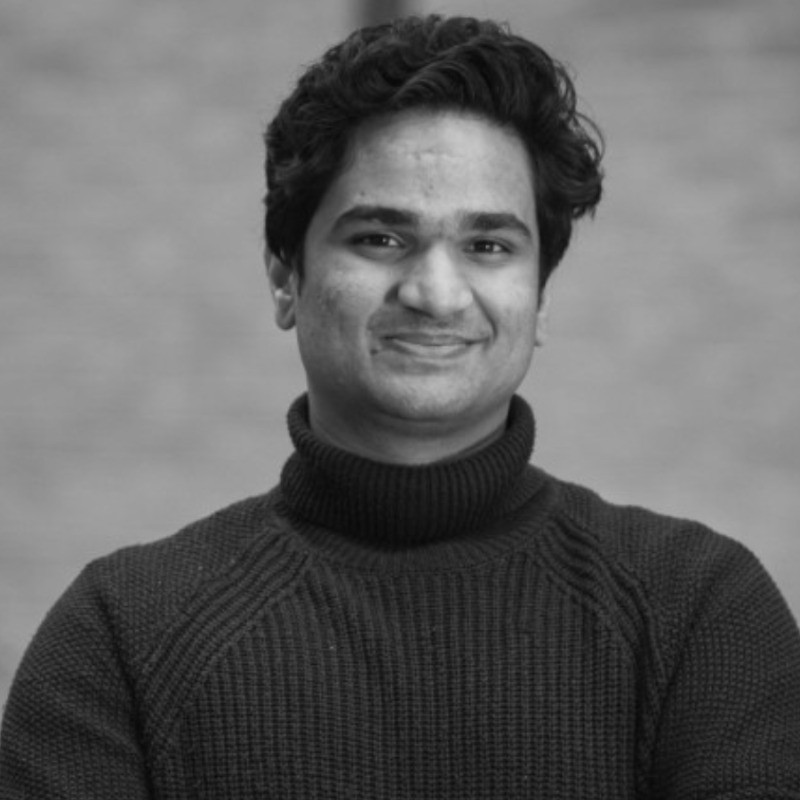
\includegraphics[width=2.0cm]{photo.jpg}
\end{minipage}
\vspace{-2pt}

% ================= SUMMARY =================
\section{Summary}
Automation QA engineer who designs test frameworks and keeps them green in CI. At FlowSpace I wrote Playwright end-to-end and API tests for a Next.js and Laravel marketplace, ran manual edge-case testing, and built an AI listing pipeline (900+ listings drafted) with validation gates.

% ================= SKILLS =================
\section{Skills}
\begin{itemize}
 \item \textbf{Test automation \& full stack:} Playwright (E2E and API tests), TypeScript, JavaScript, Node.js, Next.js, Laravel (PHP), Python, PostgreSQL, REST APIs, Docker, GitHub Actions CI
 \item \textbf{AI agents \& orchestration:} Claude Code, agentic pipelines with human-in-the-loop review, RAG, LLM data extraction, prompt engineering, Claude and OpenAI APIs, n8n, Make, agent evaluation, failure recovery
 \item \textbf{Quality \& delivery:} Test-framework design, manual and exploratory testing, CI/CD-integrated test runs, defect triage with product and engineering, third-party API integrations (OfficeRnD, Nexudus, Google, Sendgrid), production operations
\end{itemize}

% ================= EXPERIENCE =================
\section{Experience}

\role{\href{https://flowspace.co}{FlowSpace.co}}{Mar 2024 -- Aug 2026}{Full-Stack \& AI Engineer (Full-time, Freelance)}{London, UK (remote)}
\begin{itemize}
 \item Built an AI pipeline (n8n, Claude, TypeScript) that drafts workspace listings from PDF, website, photo or spreadsheet brochures, with human-in-the-loop review; 900+ listings drafted.
 \item Shipped support agents that answer customer queries against live platform data and escalate to a human on low confidence.
 \item Integrated OfficeRnD and Nexudus APIs for automated bookings, and built CRM and GTM automations for lead capture, enrichment, routing and outbound.
 \item Migrated a live marketplace off a legacy stack to coded Next.js and Laravel, scaling from 2,000 to 4,500+ users.
\end{itemize}

\role{\href{https://get2germany.com}{Get2Germany.com}}{Jan 2024 -- May 2024}{Developer \& Automation Specialist (Part-time)}{Berlin, Germany}
Integrated Google APIs, built AI tools in n8n to find courses, internships and jobs, and optimized the database.\\[1pt]

\role{\href{https://clubee.com}{Clubee.com}}{Sep 2023 -- Aug 2024}{Developer \& QA (Full-time, Freelance)}{Foetz, Luxembourg}
Integrated the Clubee API across the frontend, ran unit testing and QA, and built shop and federation-dashboard tools.\\[1pt]

\role{\href{https://tractionboard.co}{Tractionboard.co}}{Aug 2023 -- Oct 2023}{Developer (Internship)}{Utrecht, Netherlands}
Integrated ChatGPT/OpenAI and Sendgrid APIs, built responsive front-end designs, and debugged existing features.

% ================= FREELANCE PROJECTS =================
\section{Freelance Projects}
\begin{itemize}
 \item \textbf{\href{https://smarturlink.com/}{Urlink}} (2025), Project Manager \& AI-Assisted Developer. Managed client requirements, built the platform and its logic, and shipped client-driven automations. Stack: Next.js, Supabase, Netlify.
 \item \textbf{\href{https://ultrastrategy.com}{UltraStrategy}} (2024 to 2025), AI Automation Developer. Built a CV-parsing tool (LLM data extraction) with n8n and Eden AI, and a platform serving multiple user profiles.
 \item \textbf{\href{https://www.qomodo.me/}{Qomodo}} (2024 to 2025), AI Developer. Built a dashboard for companies to manage their branches, and implemented Figma designs.
\end{itemize}

% ================= CERTIFICATIONS =================
\section{Certifications}
Microsoft Copilot Studio Agent Academy \textbullet\ Microsoft: Introduction to building AI agents \textbullet\ Microsoft Power Automate \textbullet\ Tray.AI Build Practitioner (Sep 2024)

% ================= EDUCATION =================
\section{Education}
\textbf{Ca' Foscari University of Venice} \hfill Oct 2020 -- Jun 2024\\
BA Philosophy, International Studies \& Economics (Minor: Entrepreneurship)

% ================= AUTH =================
\vspace{2pt}
{\small \textbf{Work authorization:} European Long Term Residence Permit (Italy); available immediately. \quad \textbf{Languages:} Hindi (native), English (professional), Italian (beginner).}

\end{document}
